\documentclass[xcolor=dvipsnames]{beamer}

\usepackage{fontspec}
\usepackage{xunicode}
\usepackage{xltxtra}

%\setmainfont[Mapping=tex-text]{Serife Schriftart}
\setsansfont[Mapping=tex-text]{Ubuntu}
%\setmonofont[Mapping=tex-text]{Monospace Schriftart}

\mode<presentation> {
  \usetheme{default}
  \setbeamertemplate{items}{\normalsize$\bullet$}
  \usecolortheme[named=NavyBlue]{structure}
  \setbeamersize{text margin left=1cm}
}

\title{Week 2: Inspecting The Dataset}
\author{Group 4: Facial Expression Recognition}
\date{07.05.2014}

\begin{document}
\maketitle{}

\begin{frame}{Dataset overview}
  \begin{itemize}
    \item Of 593 image sequences, only 327 are labeled with emotions.
  \end{itemize}
\end{frame}

\begin{frame}{Dataset overview}
  \begin{itemize}
    \item For most AUs, no intensities are given.
    \item[] 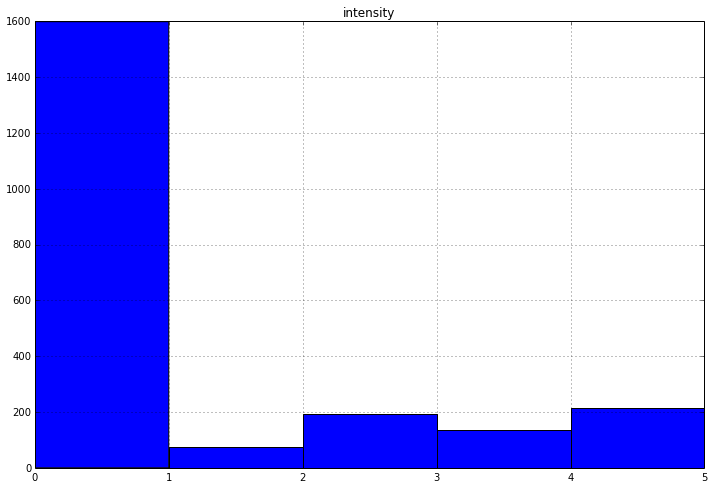
\includegraphics[width=9cm]{au_intensity_histogram}
  \end{itemize}
\end{frame}

\begin{frame}{Prediction task}
  \begin{itemize}
    \item Focus on one emotion: happiness.
    \item Predict AUs (+ maybe intensity) from landmarks.
    \item Calculate emotion from AUs according to calculation table \& verify.
    %\item[] \begin{tabular}{l|l}
    %  \textbf{Emotion} & \textbf{AUs} \\
    %  \hline
    %  Happiness & 6+12 \\
    %  \ldots
    %\end{tabular}
  \end{itemize}
  \centering
  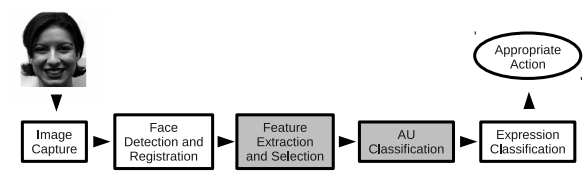
\includegraphics[width=\textwidth]{prediction_process}
\end{frame}

\begin{frame}{Prediction task}
  \begin{itemize}
    \item Find relevant landmarks for happiness.
    \item[] 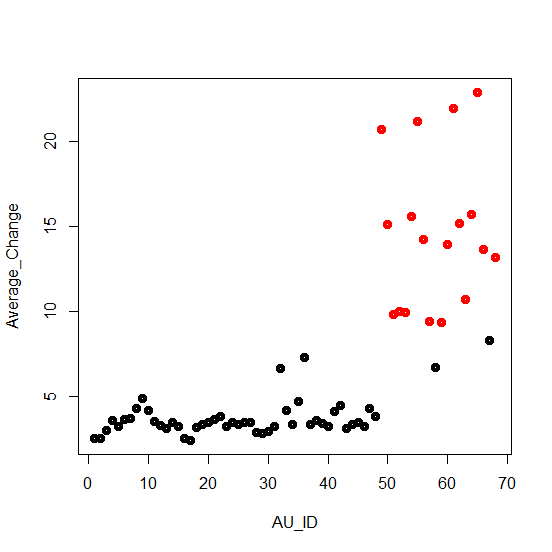
\includegraphics[height=7cm]{landmark_change}
  \end{itemize}
\end{frame}

\begin{frame}{Prediction task}
  \begin{itemize}
    \item Happy vs neutral average landmark positions.
    \item[] 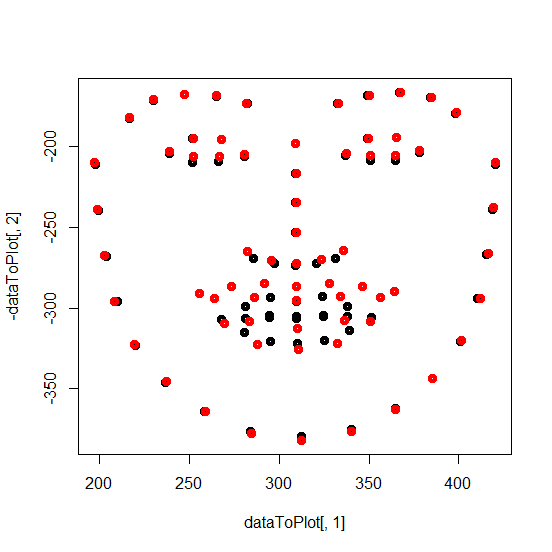
\includegraphics[height=7cm]{happy_vs_neutral}
  \end{itemize}
\end{frame}

\end{document}
